\chapter{Metodologia}
\label{chap:metodologia}

O desenvolvimento deste trabalho foi organizado em quatro frentes complementares, integradas em um único fluxo de dados que vai da aquisição do biopotencial até o monitoramento clínico: (i) um dispositivo embarcado responsável pela captura do sinal de \acs{ECG}, pelo seu processamento na borda e pela transmissão do resumo de cada segmento analisado; (ii) a infraestrutura de rede \textit{LoRaWAN}, composta por um \textit{gateway} e por um servidor de rede local; (iii) um serviço de ingestão que recebe os resumos da rede, classifica-os e os persiste em nuvem como eventos cardíacos; e (iv) um aplicativo móvel que apresenta esses eventos aos profissionais de saúde em tempo real, sinalizando como eventos de alerta aqueles de maior gravidade clínica.

Diferentemente das abordagens que transmitem a forma de onda completa do \acs{ECG}, este trabalho adotou a estratégia de \textit{processamento na borda} (\textit{edge computing}): a detecção de eventos cardíacos foi realizada no próprio dispositivo embarcado, e apenas um resumo compacto de cada segmento analisado foi transmitido pela rede \textit{LoRaWAN}. Essa decisão, detalhada na Seção~\ref{sec:transmissaoLora}, contornou as restrições de \textit{duty cycle} e de taxa de dados inerentes ao protocolo, viabilizando o monitoramento contínuo em uma rede de longo alcance e baixo consumo.

A Figura~\ref{fig:topologia} apresenta a arquitetura completa do sistema. O sinal foi captado por eletrodos conectados ao paciente, digitalizado, processado e transmitido por um sistema embarcado portátil, montado experimentalmente. O \textit{gateway} \textit{LoRaWAN} encaminhou os pacotes ao servidor de rede \textit{ChirpStack}, que os publicou em um \textit{broker} \acs{MQTT}. Um serviço de ingestão consumiu essas mensagens e gravou os eventos no banco de dados em nuvem (\textit{Firestore}), de onde o aplicativo móvel os leu em tempo real.

\begin{figure}[ht]
    \centering
    \resizebox{\linewidth}{!}{%
    \begin{tikzpicture}[
        >={Stealth[round]},
        box/.style={draw, rounded corners, align=center, minimum height=1.05cm, minimum width=2.1cm, font=\footnotesize},
        elet/.style={draw, line width=0.9pt, circle, minimum size=0.42cm, inner sep=0pt},
        lbl/.style={font=\scriptsize, align=center},
        node distance=0.9cm and 1.6cm
    ]
        % Eletrodos: três anéis empilhados verticalmente
        \node[elet] (e1) {};
        \node[elet, below=0.18cm of e1] (e2) {};
        \node[elet, below=0.18cm of e2] (e3) {};
        \foreach \n in {e1,e2,e3} { \fill (\n.center) circle (0.055); }
        \node[lbl, below=0.20cm of e3] {Eletrodos\\\acs{ECG}};

        \node[box, right=2.1cm of e2, minimum width=4.4cm, text width=4.2cm] (disp)
             {Dispositivo de aquisição e\\processamento do \acs{ECG}\\(detecção na borda)};
        \node[box, right=of disp] (gw)  {\textit{Gateway} +\\ \textit{ChirpStack}};
        \node[box, right=of gw]   (ing) {Ingestor\\(\acs{MQTT})};
        \node[box, right=of ing]  (fs)  {\textit{Firestore}\\(nuvem)};
        \node[box, below=1.0cm of fs] (app) {Aplicativo\\móvel};

        \draw[->] (e1.east) -- (disp.west);
        \draw[->] (e2.east) -- (disp.west);
        \draw[->] (e3.east) -- (disp.west);
        \draw[->] (disp) -- (gw)  node[midway, above, lbl]{\textit{LoRaWAN}};
        \draw[->] (gw)   -- (ing) node[midway, above, lbl]{\acs{MQTT}};
        \draw[->] (ing)  -- (fs);
        \draw[<->] (fs)  -- (app) node[midway, right, lbl]{\acs{SDK}};
    \end{tikzpicture}%
    }
    \caption{Topologia geral do sistema de monitoramento, da aquisição do sinal de \acs{ECG} à visualização no aplicativo móvel. A detecção ocorre no dispositivo embarcado, e apenas o resumo de cada segmento trafega pela rede.}
    \label{fig:topologia}
\end{figure}


\section{Dispositivo de Aquisição e Processamento do Sinal de ECG}
\label{sec:dispositivo}

Para a aquisição do ECG e transmissão dos eventos de alerta foram utilizados módulos comerciais de baixo custo, selecionados com o objetivo de obter um sistema compacto, confiável e energeticamente eficiente, adequado a aplicações de telemedicina e monitoramento remoto. A escolha dos componentes priorizou a alta resolução na aquisição do biopotencial, a capacidade de comunicação de longo alcance e a disponibilidade de recursos de processamento embarcado.

\subsection{Seleção dos Componentes de Hardware}
\label{sec:selecaoHardware}

A definição do microcontrolador considerou capacidade de processamento, conectividade, consumo energético, dimensões e custo. Optou-se pelo módulo XIAO ESP32-S3, que reúne, em um encapsulamento de dimensões reduzidas (21~$\times$~17,5~mm), um processador de dois núcleos, suporte nativo a \textit{Wi-Fi} e \textit{Bluetooth}, controlador de recarga de bateria (íons de lítio) integrado e memória \textit{PSRAM} de 8~MB. Esse último recurso foi determinante para o projeto, pois permitiu armazenar em memória os segmentos de 30~s de sinal necessários ao algoritmo de detecção. A Tabela~\ref{tab:mcu} compara o módulo escolhido com o Arduino~Uno, plataforma recorrente em trabalhos correlatos.

\begin{table}[h]
    \centering
    \caption{Comparativo entre os microcontroladores avaliados.}
    \begin{tabular}{l|>{\centering\arraybackslash}m{3.2cm}|>{\centering\arraybackslash}m{3.2cm}}
         & \textbf{XIAO ESP32-S3} & \textbf{Arduino Uno} \\ \hline
        \textbf{Núcleo} & \textit{Xtensa} LX7 \mbox{dual-core} 32 bits & ATmega328P 8 bits \\ \hline
        \textbf{Frequência} & até 240 MHz & 16 MHz \\ \hline
        \textbf{Memória} & 512 KB SRAM + 8 MB PSRAM & 2 KB SRAM \\ \hline
        \textbf{Conectividade} & \textit{Wi-Fi} + \textit{Bluetooth}/BLE & nenhuma nativa \\ \hline
        \textbf{Bateria} & controlador de carga integrado & externo \\ \hline
        \textbf{Dimensões} & 21 $\times$ 17,5 mm & 68,6 $\times$ 53,4 mm \\ \hline
        \textbf{Preço aproximado \acs{FOB}} & USD 9,90 & USD 11,90 \\ \hline
    \end{tabular}
    \label{tab:mcu}
\end{table}

Para a aquisição do sinal de ECG, a revisão bibliográfica evidenciou que a maioria dos trabalhos emprega o módulo AD8232. Esse componente, contudo, apresenta limitações relevantes: não dispõe de conversor analógico-digital (A/D) integrado, exigindo o uso do \acs{ADC} interno do microcontrolador, cuja resolução efetiva (10--12 bits) e taxa de amostragem são limitadas; além disso, oferece uma única derivação \citep{AnalogDevices_AD8232}. Optou-se, portanto, pelo módulo CJMCU-1293, baseado no \acs{AFE} ADS1293, que integra três canais simultâneos, conversão de 24~bits e taxa de amostragem programável \citep{TexasInstruments_ADS1293}. A Tabela~\ref{tab:ads_vs_ad8232} sintetiza as vantagens do módulo adotado.

\begin{table}[h]
    \centering
    \caption{Comparativo entre os \acs{AFE} ADS1293 e AD8232 para aplicações em \acs{ECG}.}
    \begin{tabular}{l|>{\centering\arraybackslash}m{4.5cm}|>{\centering\arraybackslash}m{4.5cm}}
         & \textbf{ADS1293 (CJMCU-1293)} & \textbf{AD8232} \\ \hline
        \textbf{Conversor A/D} & 24 bits & Não possui (saída analógica) \\ \hline
        \textbf{Canais} & Até 3 canais simultâneos & 1 canal \\ \hline
        \textbf{Taxa de amostragem} & Programável (até 25,6 kSPS) & Definida pelo microcontrolador externo \\ \hline
        \textbf{Resolução efetiva} & 24 bits nativos & 10--12 bits (ADC do MCU) \\ \hline
        \textbf{Consumo de energia} & 0,3 mW por canal & Muito baixo (depende do circuito externo) \\ \hline
        \textbf{Recursos para ECG} & RLD, detecção de eletrodo solto, filtros programáveis & RLD, detecção de eletrodo solto \\ \hline
        \textbf{Aplicação típica} & ECG portátil de alta precisão; pesquisa biomédica & Ensino, prototipagem, \textit{wearables} simples \\ \hline
    \end{tabular}
    \label{tab:ads_vs_ad8232}
\end{table}

A transmissão dos dados coube ao módulo \textit{LoRa} Wio-SX1262, escolhido pela comunicação de longo alcance e pelo baixo consumo característicos da tecnologia. A alimentação do conjunto foi provida por uma bateria de íons de lítio de 3,7~V. 

\subsection{Arquitetura e Funcionamento do Dispositivo}
\label{sec:arqDispositivo}

O ADS1293 registra os sinais bioelétricos do coração e os transfere já digitalizados ao microcontrolador por meio de um barramento \acs{SPI} (\textit{Serial Peripheral Interface}). A Tabela~\ref{tab:pinagem} apresenta a pinagem utilizada na interligação entre o ADS1293 e o XIAO ESP32-S3. O sinal de interrupção \acs{DRDY} (\textit{Data Ready}) foi empregado para sinalizar, a cada nova amostra disponível, a leitura pelo microcontrolador, garantindo a aquisição em taxa constante.

\begin{table}[h]
    \centering
    \caption{Pinagem da interface \acs{SPI} entre o ADS1293 e o XIAO ESP32-S3.}
    \begin{tabular}{l|c|l}
        \textbf{Sinal} & \textbf{Pino XIAO} & \textbf{Função} \\ \hline
        DRDY & D1 & Interrupção: amostra pronta \\ \hline
        CS   & D3 & \textit{Chip Select} \\ \hline
        SCK  & D8 & \textit{Clock} \acs{SPI} \\ \hline
        MISO & D9 & \textit{Master In, Slave Out} \\ \hline
        MOSI & D10 & \textit{Master Out, Slave In} \\ \hline
    \end{tabular}
    \label{tab:pinagem}
\end{table}

A Figura~\ref{fig:conexoes} mostra a interligação completa entre os módulos. A comunicação com o ADS1293 emprega sete conexões: cinco de natureza digital e duas de alimentação. As linhas digitais compreendem o barramento \acs{SPI} propriamente dito — \textit{clock} (SCK), dados do microcontrolador para o \acs{AFE} (MOSI, ligado ao pino SDI do módulo), dados do \acs{AFE} para o microcontrolador (MISO, ligado ao pino SDO) e seleção de dispositivo (CS, ligado ao pino CSB) — acrescidas do sinal de interrupção \acs{DRDY} (pino DRDYB), que sinaliza cada nova amostra disponível. As duas conexões restantes são a alimentação de 3,3~V e o GND.

Quanto à energia, o conjunto é alimentado por uma bateria de íons de lítio de 3,7~V, modelo 18650 (18~mm de diâmetro por 65~mm de comprimento) conectada diretamente aos terminais de bateria (BAT) do XIAO ESP32-S3; o regulador interno do microcontrolador disponibiliza os 3,3~V que alimentam o ADS1293, respeitando o limite de tensão analógica (\textit{AVDD}) de 3,6~V do componente. A porta USB-C destina-se exclusivamente à recarga da bateria, não alimentando o circuito durante a operação. O módulo \textit{LoRa} Wio-SX1262, por sua vez, ocupa um barramento \acs{SPI} dedicado, com pinos internos distintos, o que elimina conflito de comunicação com o \acs{AFE}.

\begin{figure}[htb]
\centering
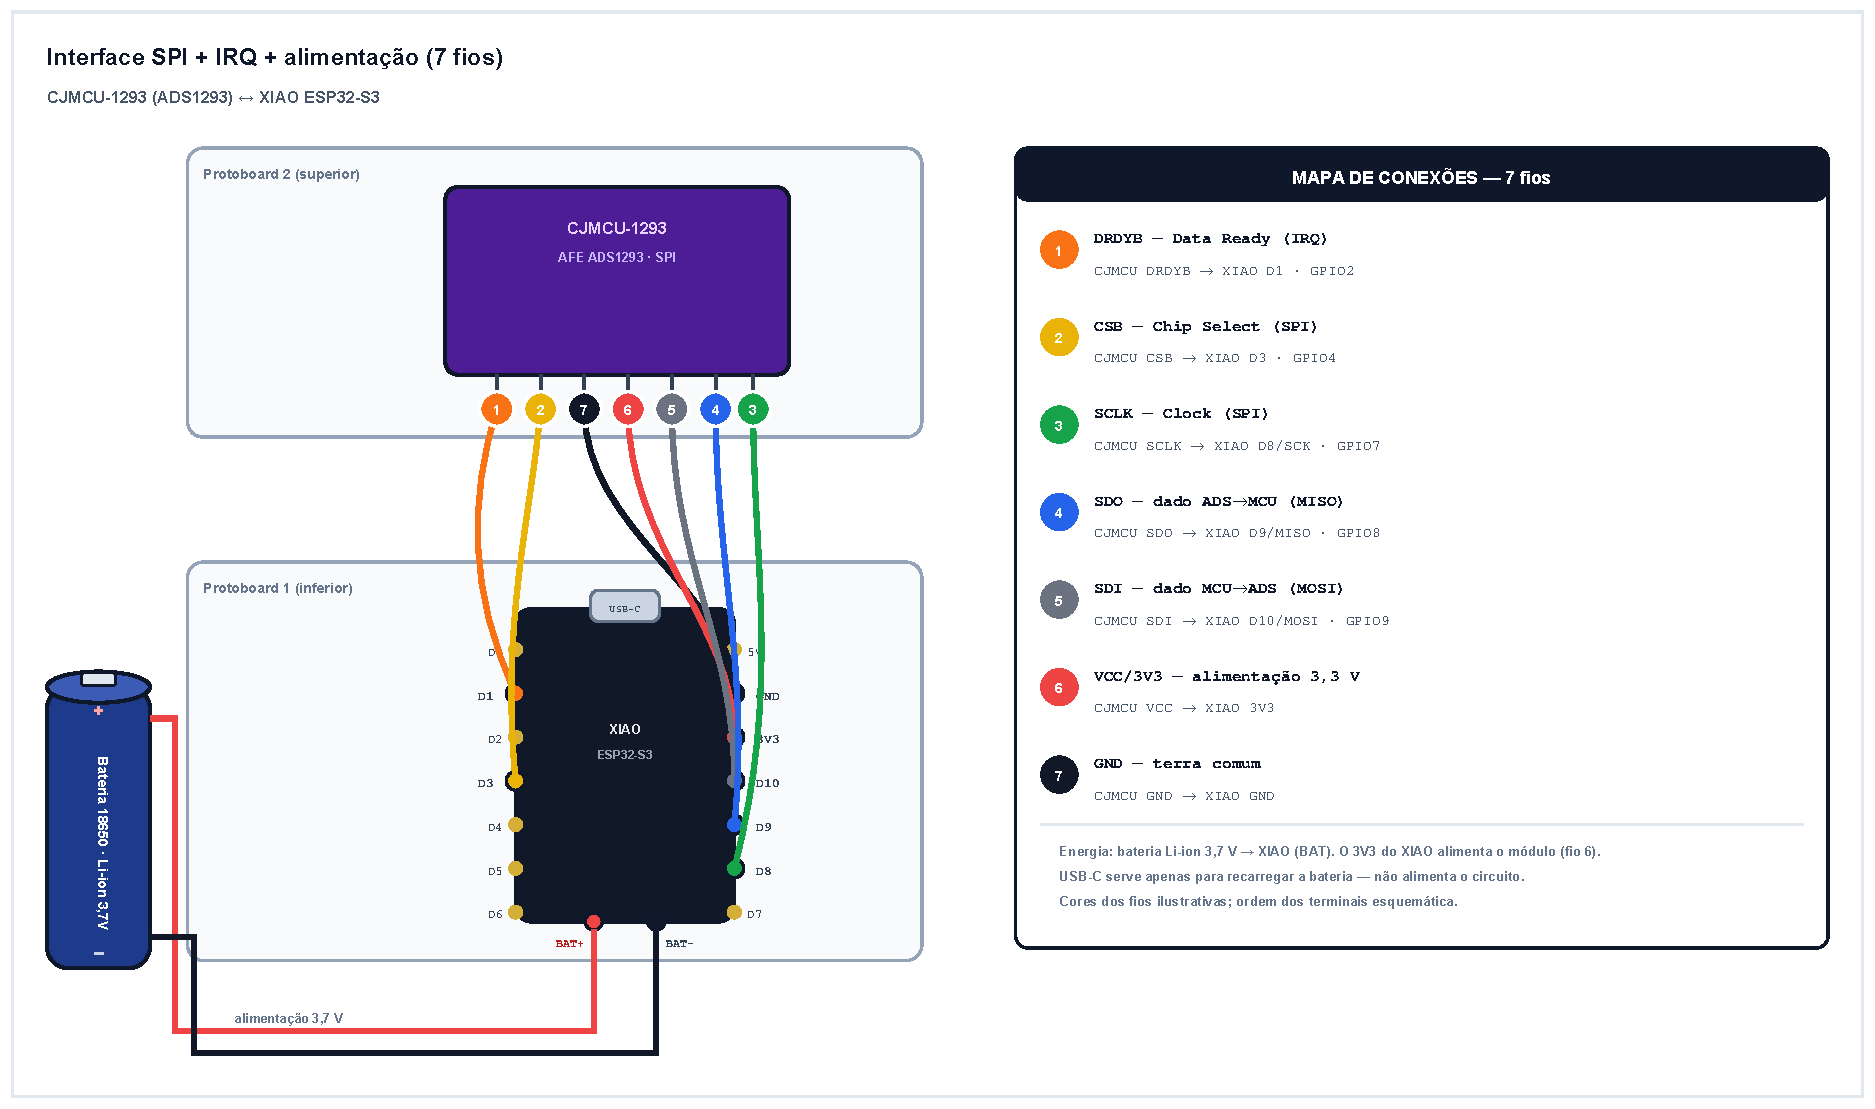
\includegraphics[width=0.95\textwidth]{assets/diagrama_conexoes.pdf}
\caption{Diagrama de conexões do protótipo: interface \acs{SPI} e interrupção entre o \acs{AFE} CJMCU-1293 (ADS1293) e o XIAO ESP32-S3, alimentação a partir da bateria de íons de lítio e recarga por USB-C. As cores dos condutores são ilustrativas.}
\label{fig:conexoes}
\end{figure}

A aquisição foi realizada segundo o triângulo de \textit{Einthoven}, obtendo-se três derivações a partir dos 3 eletrodos fixados no tórax. As derivações I e II foram medidas diretamente pelos canais 1 e 2 do ADS1293, e a derivação III foi calculada por meio da lei de \textit{Einthoven}, conforme as Equações~\ref{eq:leadI} a~\ref{eq:leadIII}:

\begin{align}
    \text{Derivação I}   &= \text{LA} - \text{RA} \label{eq:leadI} \\
    \text{Derivação II}  &= \text{LL} - \text{RA} \label{eq:leadII} \\
    \text{Derivação III} &= \text{Derivação II} - \text{Derivação I} \label{eq:leadIII}
\end{align}

\noindent em que RA, LA e LL representam, respectivamente, os eletrodos do braço direito, do braço esquerdo e da perna esquerda. A derivação II foi adotada como referência para o algoritmo de detecção, por apresentar, tipicamente, a maior amplitude do complexo QRS. A Figura~\ref{fig:diagrama_ecg} ilustra o diagrama de blocos do dispositivo.

\begin{figure}[ht]
    \centering
    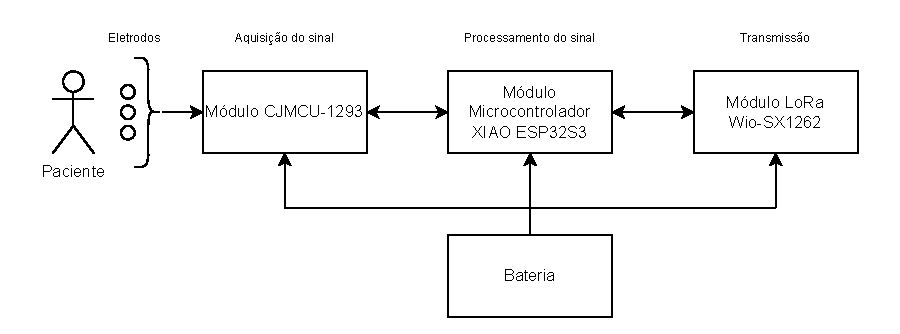
\includegraphics[width=1\linewidth]{assets/blocosDispositivoHardware.drawio.pdf}
    \caption{Diagrama de blocos do dispositivo de aquisição e transmissão do sinal de \acs{ECG}.}
    \label{fig:diagrama_ecg}
\end{figure}


\subsection{Módulo de Comunicação Wio-SX1262}
\label{sec:sx1262}

O Wio-SX1262 é um módulo \textit{LoRa} baseado no transceptor \textit{Semtech} SX1262, projetado para transmissões de longo alcance e baixo consumo. Suas principais características, conforme o fabricante \citep{WioSX1262Datasheet}, são:

\begin{itemize}
    \item \textbf{Consumo em repouso}: 1,62 µA em modo \textit{sleep}.
    \item \textbf{Frequência de operação}: 862--930 MHz, abrangendo as principais regulamentações regionais do \textit{LoRaWAN}.
    \item \textbf{Potência de transmissão}: até 22 dBm (158 mW).
    \item \textbf{Sensibilidade de recepção}: até -136,73 dBm (SF12, largura de banda de 125 kHz).
    \item \textbf{Interfaces}: comunicação \acs{SPI} com o microcontrolador e conector \acs{IPEX} para antena externa.
\end{itemize}

No XIAO ESP32-S3, o Wio-SX1262 ocupa um barramento \acs{SPI} dedicado, com pinos internos distintos dos utilizados pelo ADS1293, eliminando conflitos de comunicação entre os dois periféricos.

\subsection{Módulo de Aquisição CJMCU-1293 (ADS1293)}
\label{sec:cjmcu}

O CJMCU-1293 é um módulo de desenvolvimento que integra o \acs{AFE} (\textit{Analog Front End}) ADS1293, circuito integrado de baixo consumo projetado para aplicações médicas portáteis. Suas principais características são:

\begin{itemize}
    \item \textbf{Arquitetura e precisão}: 3 canais de alta resolução para aquisição simultânea de \acs{ECG}; conversão A/D de 24 bits; taxa de amostragem programável de até 25,6 kSPS.
    \item \textbf{Consumo de energia}: 0,3 mW por canal, com modos de baixo consumo e \textit{standby}.
    \item \textbf{Faixa de operação}: alimentação analógica de 2,7 V a 5,5 V e entrada diferencial de ±400 mV, compatível com eletrodos de \acs{ECG} comuns.
    \item \textbf{Funcionalidades para ECG}: detecção de eletrodo desconectado (\textit{Lead-Off Detection}); entradas com imunidade a interferência eletromagnética (\textit{EMI-Hardened Inputs}); e amplificador de perna direita (\textit{Right-Leg Drive} -- RLD), que reduz o ruído de modo comum, em especial a interferência de 60 Hz da rede elétrica.
    \item \textbf{Interface}: comunicação via \acs{SPI} com o microcontrolador.
\end{itemize}

A configuração do ADS1293 foi realizada para operação em três derivações (\textit{3-Lead}), com a detecção de modo comum e o amplificador RLD habilitados, condições necessárias à obtenção de um sinal limpo durante a movimentação do paciente.

Em uma aplicação convencional, o amplificador RLD requer um quarto eletrodo, posicionado na perna direita do paciente, para o qual o sinal de contrarreação de modo comum é aplicado. Com o objetivo de reduzir o número de cabos e simplificar a montagem, optou-se por dispensar esse eletrodo dedicado e adotar uma topologia de \textit{driven-leg} com apenas três eletrodos, na qual as funções de detecção e de contrarreação do modo comum são atribuídas a eletrodos distintos.

A detecção de modo comum, realizada pelo \textit{Common-Mode Detector} do ADS1293, calcula a média das tensões dos pinos de entrada habilitados no registrador \texttt{CMDET\_EN} \citep{TexasInstruments_ADS1293}. Habilitaram-se apenas os pinos IN1 e IN3 (\texttt{CMDET\_EN = 0x05}), correspondentes aos eletrodos do braço direito (RA) e da perna esquerda (LL), deixando o eletrodo do braço esquerdo (LA) livre para receber a contrarreação. O roteamento da saída do RLD, por sua vez, é definido pelos três bits menos significativos (campo \textit{SELRLD}) do registrador \texttt{RLD\_CN}: enquanto o valor padrão da biblioteca de controle (\texttt{SELRLD = 100}) direciona a saída ao pino IN4 (eletrodo de perna direita), o valor adotado neste trabalho (\texttt{SELRLD = 010}) a direciona ao pino IN2, associado ao eletrodo LA. Dessa forma, a média de modo comum é obtida de RA e LL e reinjetada por LA, mantendo-se a separação entre os eletrodos de detecção e de contrarreação característica da topologia clássica de \textit{driven-leg} e obtendo-se a atenuação do ruído de modo comum de 60~Hz com apenas três eletrodos. A taxa de conversão foi definida pelos registradores de decimação \texttt{R2} e \texttt{R3}, programados por meio da configuração \texttt{SPS\_256} da biblioteca de controle, o que resulta na taxa efetiva de 640 amostras por segundo por canal --- valor verificado experimentalmente e adotado em todo o processamento subsequente.


\section{Firmware Embarcado}
\label{sec:firmware}

O \textit{firmware} do dispositivo foi desenvolvido em C++ sobre a plataforma \textit{Arduino}, e estruturado em torno de um laço orientado a interrupção: a cada borda do sinal \acs{DRDY}, uma amostra das três derivações foi lida do ADS1293 acumulada em um \textit{buffer}. Ao completar um segmento de 30~s, o algoritmo de detecção de arritmias foi executado, o resultado foi registrado em memória não volátil e, então, transmitido pela rede \textit{LoRaWAN}.

\subsection{Aquisição e Condicionamento do Sinal}
\label{sec:condicionamento}

As amostras brutas, fornecidas pelo conversor de 24 bits, foram convertidas para a escala de tensão segundo a Equação~13 do manual do componente \citep{TexasInstruments_ADS1293}, $v = \left(raw/\mathrm{ADC_{MAX}} - 1/2\right)\cdot 2V_{ref}/G$, em que $G = 3{,}5$ é o ganho do amplificador de instrumentação, $V_{ref} = 2{,}4$~V é a referência interna e $\mathrm{ADC_{MAX}}$ é o fundo de escala do conversor. Cabe observar que esse fundo de escala não corresponde à excursão total de 24 bits: ele é determinado pelas razões de decimação programadas em \texttt{R2} e \texttt{R3}, valendo $\mathrm{ADC_{MAX}} = \mathtt{0xC35000}$ na configuração adotada, e a saída é codificada em binário com \textit{offset}, de modo que a meia escala corresponde a 0~V diferencial. Em seguida, cada derivação foi submetida a uma cascata de dois filtros digitais de resposta ao impulso infinita (\acs{IIR}): um filtro passa-baixas, com frequência de corte de 40 Hz, para atenuar o ruído muscular e a interferência da rede elétrica; e um filtro passa-altas, com frequência de corte de 0,5 Hz, para remover o desvio de linha de base (\textit{baseline wander}) e a componente contínua de \textit{offset} dos eletrodos. Ambos os filtros são de primeira ordem: o passa-baixas na forma de média móvel exponencial e o passa-altas na forma canônica de um polo, com coeficientes $\alpha \approx 0{,}3247$ e $\alpha \approx 0{,}9951$, respectivamente. Optou-se pela estrutura \acs{IIR}, em detrimento de um filtro \acs{FIR} de fase linear, pelo custo computacional: um \acs{FIR} equivalente, projetado por janelamento de \textit{Hamming}, exigiria da ordem de $3{,}3\,f_s/\Delta f$ coeficientes --- algumas centenas para o corte de 40~Hz e alguns milhares para o de 0,5~Hz ---, contra uma única multiplicação-acumulação e um estado por amostra na estrutura adotada, em um microcontrolador que executa concomitantemente a aquisição, o armazenamento do segmento e a pilha \textit{LoRaWAN}. A distorção de fase decorrente concentra-se abaixo de 2~Hz e afeta sobretudo o segmento ST e a onda T, e não a localização temporal do complexo QRS, da qual dependem as grandezas efetivamente medidas pelo sistema; ademais, o realce do QRS no algoritmo de detecção (Seção~\ref{sec:deteccaoBorda}) é realizado por um filtro janela-sinc, de fase linear. Os coeficientes foram calculados para a taxa de amostragem do sistema, de 640~SPS, decorrente das razões de decimação programadas no conversor (Equação~\ref{eq:odr}) e suficiente, com ampla margem, para a banda de interesse do sinal, limitada a 40~Hz pelo próprio passa-baixas. Cabe registrar que essa taxa não corresponde ao valor nominal sugerido pela nomenclatura da configuração empregada na biblioteca de controle, discrepância identificada durante a caracterização do componente e detalhada no Capítulo~\ref{chap:resultados}.

A saída de depuração pela interface serial foi desacoplada da aquisição, de modo a preservar a integridade temporal do sinal processado. A interface opera a 230.400 bits por segundo e cada amostra impressa ocupa cerca de 42 caracteres, com as três derivações em representação textual; a 640 amostras por segundo, a vazão exigida é de aproximadamente 270~kbit/s, acima da capacidade do enlace. Excedida essa capacidade, a operação de escrita bloqueia o laço principal enquanto o \textit{buffer} de transmissão se esvazia, o que ocasiona a perda de interrupções \acs{DRDY}, introduz descontinuidades no \textit{buffer} de detecção e distorce os intervalos R-R. Para evitá-lo, a saída de depuração foi decimada — apenas uma a cada quatro amostras é enviada à serial, o que reduz a vazão exigida a cerca de 67~kbit/s —, enquanto o \textit{buffer} de detecção continuou a receber todas as amostras. Nas coletas automatizadas, em que apenas as linhas de resumo interessam, a impressão de amostras foi inteiramente desativada. Preservou-se, assim, a visualização em tempo real sem comprometer o sinal efetivamente submetido à detecção.

\subsection{Detecção de Eventos na Borda}
\label{sec:deteccaoBorda}

O núcleo do processamento embarcado consistiu em um algoritmo de detecção de complexos QRS e de classificação de arritmias, aplicado à derivação II de cada segmento de 30~s. Esse algoritmo não é uma contribuição deste trabalho: trata-se do \textit{firmware} de detecção desenvolvido por \citeay{moraesFirmwareECG}, descrito na Seção~\ref{sec:deteccaoEmbarcada}, cujo código-fonte foi cedido pelos autores e aqui reutilizado. 

A adaptação realizada limitou-se ao necessário para a execução na plataforma adotada: ajuste da taxa de amostragem (de 500 para 640~SPS, com a consequente reescrita dos limiares expressos em número de amostras por unidade de tempo), e integração ao \textit{buffer} de aquisição e ao \textit{payload} de transmissão. As regras de decisão dos limiares clínicos passaram por ajustes sutis, de modo a manter a comparabilidade com os resultados originais.

O algoritmo, baseado na análise da derivada do sinal --- método da operação de diferenças (DOM, \textit{Difference Operation Method}) ---, seguiu as etapas:

\begin{enumerate}
    \item \textbf{Diferenciação}: cálculo da diferença discreta entre amostras consecutivas, realçando as transições rápidas associadas ao complexo QRS.
    \item \textbf{Filtragem}: filtragem do sinal diferenciado com um filtro passa-baixas do tipo janela-sinc, suavizando as componentes de alta frequência remanescentes.
    \item \textbf{Limiarização adaptativa}: cálculo de limiares positivo e negativo proporcionais à média das amplitudes de cada polaridade, separando os extremos significativos do ruído de fundo.
    \item \textbf{Pareamento e detecção de picos}: identificação dos pares de extremos (descida e subida) correspondentes a cada complexo QRS e localização dos picos R.
    \item \textbf{Cálculo dos intervalos R-R}: a partir das posições dos picos R, foram obtidos os intervalos R-R e suas estatísticas (média, desvio padrão e diferenças sucessivas), base para a classificação. Essas estatísticas correspondem aos índices de variabilidade da frequência cardíaca no domínio do tempo padronizados por \citeay{hrvTaskForce1996}.
\end{enumerate}


Com base nas estatísticas dos intervalos R-R, o algoritmo classifica o segmento em seis categorias de anormalidade: taquicardia, bradicardia, arritmia sinusal, bloqueio sinoatrial, parada sinoatrial e anomalia não caracterizada. As cinco primeiras provêm do trabalho de \cite{moraesFirmwareECG}; a sexta foi acrescentada neste trabalho e é descrita adiante. A taquicardia é sinalizada quando o intervalo R-R médio é inferior a 600 ms (frequência cardíaca acima de 100 bpm) e a bradicardia quando superior a 1000 ms (abaixo de 60 bpm).

A arritmia sinusal é sinalizada quando a diferença entre dois intervalos R-R consecutivos situa-se entre 120 ms e 80\,\% do intervalo R-R de base. O limite superior não constava da formulação original e foi acrescentado para impedir que a diferença produzida por uma pausa fosse contabilizada também como variabilidade sinusal. Assim, o contador de arritmia passa a representar variações batimento a batimento, enquanto os intervalos longos são avaliados pelos critérios de pausa descritos a seguir.

As duas classes de pausa foram decididas em relação ao ritmo de base do próprio segmento, e não por duração absoluta. No bloqueio sinoatrial de segundo grau, a pausa corresponde a dois ou três intervalos R-R do ritmo de base; na parada sinusal, a pausa excede três intervalos R-R. Adotou-se como ritmo de base a mediana dos intervalos R-R do segmento, por ser menos sensível ao próprio intervalo pausado do que a média. A comparação do bloqueio com os múltiplos de dois e três ciclos admitiu tolerância relativa de 5\,\%, considerando a variabilidade fisiológica e as não idealidades do registro. Não se impôs piso de duração absoluta: a uma frequência cardíaca elevada, uma pausa de dois intervalos R-R é breve em termos absolutos, mas continua sendo, por definição, um bloqueio.

A sexta categoria --- anomalia não caracterizada --- foi acrescentada para cobrir os segmentos em que há evidência de anormalidade no ritmo, mas que não corresponde a nenhuma das cinco alterações detectadas. Sinaliza-se essa categoria quando um intervalo de pelo menos uma vez e meia o R-R de base não satisfaz os critérios de arritmia sinusal, bloqueio ou parada. Na prática, ela cobre a descontinuidade entre as faixas: intervalos longos demais para serem tratados como variabilidade sinusal, mas que não se aproximam de dois ou três ciclos e tampouco excedem três ciclos. Trata-se de uma classe residual; ela não substitui a detecção de bloqueio ou parada quando esses critérios são satisfeitos, nem cria um diagnóstico novo.

A justificativa para acrescentar uma categoria, em vez de estender as faixas dos critérios existentes, é de natureza clínica. Alargar o critério de bloqueio para abranger durações intermediárias faria o sistema indicar alterações falsas (falsos positivos). A categoria adicional indica que há anormalidade e que ela não é caracterizável pelos critérios usados atualmente, conduta apropriada a um monitor de triagem, cuja finalidade é encaminhar o paciente para exames mais detalhados. Quando a máscara de \textit{bits} precisa ser convertida em um único rótulo, a anomalia não caracterizada fica por último na ordem de prioridade, pois só deve aparecer como classificação principal quando nenhuma alteração específica foi detectada.

Registre-se que a formulação relativa das pausas, o teto do critério de arritmia e a categoria adicional foram as adaptações de regra de decisão incorporadas neste trabalho ao algoritmo de \citet{moraesFirmwareECG}. Essas adaptações foram conduzidas sob orientação dos autores do algoritmo, com o objetivo de adequar a classificação ao uso no protótipo desenvolvido e de preservar, no registro transmitido, informações úteis à triagem. Suas consequências experimentais são reportadas na Seção~\ref{sec:resValidacaoFinal}.

O resultado primário da classificação é a máscara de \textit{bits}, de modo que mais de uma alteração pode permanecer registrada no mesmo segmento. Taquicardia, bradicardia, arritmia sinusal, bloqueio, parada e anomalia não caracterizada não são mutuamente excludentes no resumo gravado. A ordem de prioridade é aplicada apenas depois, na etapa de ingestão, quando a máscara precisa ser representada por um único tipo de evento para indexação e apresentação no sistema (Seção~\ref{sec:resPipeline}).

Para evitar resultados indevidos, segmentos com menos de três picos R detectados foram marcados como erro de processamento. Esse limite é operacional: com menos de três picos há, no máximo, um intervalo R-R, quantidade insuficiente para calcular diferenças sucessivas entre intervalos e aplicar os critérios temporais da classificação. Essa condição não equivale à classe normal nem à anomalia não caracterizada. A classe normal corresponde ao segmento com picos suficientes e sem critérios de anormalidade satisfeitos; a anomalia não caracterizada, por sua vez, exige picos suficientes e ao menos um intervalo longo que não se enquadre nas classes nomeadas. A Tabela~\ref{tab:criteriosClassificacao} resume os critérios aplicados a cada segmento.

\begin{table}[H]
    \centering
    \caption{Critérios de classificação aplicados aos intervalos R-R de cada segmento.}
    \label{tab:criteriosClassificacao}
    \small
    \setlength{\tabcolsep}{4pt}
    \renewcommand{\arraystretch}{1.08}
    \begin{tabular}{>{\raggedright\arraybackslash}p{3.6cm}>{\raggedright\arraybackslash}p{5.1cm}>{\raggedright\arraybackslash}p{5.0cm}}
        \hline
        \textbf{Condição} & \textbf{Critério} & \textbf{Observação} \\ \hline
        Erro de processamento & Menos de três picos R detectados & Não há intervalos suficientes para aplicar os critérios temporais; o segmento é mantido apenas no registro local. \\ \hline
        Taquicardia & $\overline{RR} < 600$ ms & Equivale a frequência cardíaca média acima de 100 bpm. \\ \hline
        Bradicardia & $\overline{RR} > 1000$ ms & Equivale a frequência cardíaca média abaixo de 60 bpm. \\ \hline
        Arritmia sinusal & $120$ ms $< |\Delta RR| < 0{,}8\,\widetilde{RR}$ & Conta variações batimento a batimento; o teto evita contabilizar pausas como variabilidade sinusal. \\ \hline
        Bloqueio sinoatrial & $RR_i \approx 2\widetilde{RR}$ ou $RR_i \approx 3\widetilde{RR}$, com tolerância de 5\,\% & Pausa de dois ou três ciclos do ritmo de base. \\ \hline
        Parada sinusal & $RR_i > 3(1+0{,}05)\widetilde{RR}$ & Pausa superior a três ciclos do ritmo de base. \\ \hline
        Anomalia não caracterizada & $RR_i \ge 1{,}5\widetilde{RR}$ sem satisfazer os critérios de arritmia sinusal, bloqueio ou parada & Classe residual para intervalo longo não enquadrado nas classes nomeadas. \\ \hline
    \end{tabular}
\end{table}

\subsection{Armazenamento Local}
\label{sec:armazenamento}

Para conferir robustez ao sistema diante de eventuais falhas de comunicação e permitir a validação posterior dos dados, o \textit{firmware} mantem um registro local em memória \textit{flash}, por meio do sistema de arquivos \textit{LittleFS}. Para cada segmento de 30~s, independentemente de sua classificação, é gravado um resumo compacto de 16 bytes contendo o identificador sequencial do segmento, a frequência cardíaca estimada, o intervalo R-R médio e seu desvio padrão, o número de picos detectados e as anormalidades identificadas. O registro local reúne os mesmos campos do \textit{payload} transmitido (Tabela~\ref{tab:payload}), acrescidos do instante de conclusão do processamento, em 4 bytes, e com o identificador do segmento em 32 bits, e não em 16. Daí a diferença entre os 16 bytes gravados e os 10 transmitidos: a gravação em memória \textit{flash} não consome tempo de ocupação do canal, de modo que não há por que truncar os campos, ao passo que no enlace \textit{LoRaWAN} cada byte acrescenta tempo no ar. Adicionalmente, para os segmentos classificados como anormais, o sinal bruto da derivação II foi armazenado integralmente, possibilitando a inspeção \textit{a posteriori} da forma de onda associada ao evento. Foram implementadas políticas de rotação que descartam os registros mais antigos quando o espaço disponível na memória \textit{flash} se aproxima do limite reservado ao armazenamento local, garantindo a operação contínua do dispositivo sem interrupção por falta de espaço.

\subsection{Transmissão via LoRaWAN}
\label{sec:transmissaoFirmware}
\label{sec:transmissaoLora}

A transmissão empregou a biblioteca \textit{RadioLib} (versão 7.1.2) e o protocolo \textit{LoRaWAN} na região AU915 (sub-banda 2), com ativação por \acs{OTAA} (\textit{Over-the-Air Activation}) e operação em Classe~A. Ao final de cada segmento de 30~s do sinal de \acs{ECG}, foi enviado, na porta de aplicação 2, um \textit{payload} de 10 bytes contendo o resumo transmitido do segmento, codificado em formato \textit{big-endian}, conforme a Tabela~\ref{tab:payload}. Esse \textit{payload} é menor que o registro local de 16 bytes porque omite o instante de processamento gravado na memória \textit{flash} e transmite apenas os 16 bits menos significativos do identificador sequencial do segmento. O reduzido tamanho do \textit{payload} foi resultado direto da estratégia de detecção na borda e constituiu o elemento central que viabilizou a transmissão sobre \textit{LoRaWAN}.

Um aspecto prático da ativação por \acs{OTAA} exigiu tratamento específico. A cada reinicialização do dispositivo, o contador de segurança do protocolo de ingresso (\textit{DevNonce}) é reiniciado; como o servidor de rede rejeita valores de \textit{DevNonce} já utilizados, para prevenir ataques de repetição, cada reinício resultava na recusa do ingresso até a limpeza manual dos \textit{nonces} no \textit{ChirpStack}. Para eliminar essa dependência de intervenção, o estado do enlace foi persistido na memória não volátil do microcontrolador (\textit{Non-Volatile Storage} -- NVS, do ESP32): tanto os \textit{nonces} de ingresso quanto o contexto da sessão (chaves derivadas e contadores de quadro) são gravados após cada ativação bem-sucedida e a cada \textit{uplink}. Na inicialização, esse estado é restaurado antes da ativação, o que permite ao dispositivo retomar a sessão existente sem repetir o procedimento de ingresso ou, quando um novo ingresso é necessário, apresentar um \textit{DevNonce} sempre crescente. Dessa forma, o dispositivo tolera reinícios e quedas de energia sem intervenção no servidor de rede, requisito essencial para operação autônoma prolongada.

\begin{table}[h]
    \centering
    \caption{Estrutura do \textit{payload} de 10 bytes transmitido via \textit{LoRaWAN}.}
    \begin{tabular}{c|l|c}
        \textbf{Byte(s)} & \textbf{Campo} & \textbf{Tipo} \\ \hline
        0 & \textit{Flags} de detecção (\textit{bitmask}) & uint8 \\ \hline
        1--2 & Frequência cardíaca (bpm) & uint16 \\ \hline
        3--4 & Intervalo R-R médio (ms) & uint16 \\ \hline
        5--6 & Desvio padrão do R-R (ms) & uint16 \\ \hline
        7 & Número de picos R & uint8 \\ \hline
        8--9 & Identificador do segmento & uint16 \\ \hline
    \end{tabular}
    \label{tab:payload}
\end{table}

O campo de desvio padrão do R-R corresponde ao índice \acs{SDNN} --- desvio padrão dos intervalos entre batimentos --- tal como definido por \citeay{hrvTaskForce1996}, calculado, neste trabalho, sobre a janela de 30~s de cada segmento. Cabe registrar que essa janela é inferior aos 5~min mínimos preconizados naquele documento para os registros curtos, e que os batimentos ectópicos não são excluídos da série antes do cálculo; o valor transmitido presta-se, portanto, à caracterização da dispersão dos intervalos dentro do segmento, e não à comparação direta com os índices de variabilidade reportados na literatura clínica.


O campo de \textit{flags} codificou, em uma máscara de bits, as seis categorias de anormalidade, permitindo o registro de detecções simultâneas em um mesmo segmento. O identificador sequencial do segmento possibilitou ao servidor detectar eventuais perdas de pacotes. A aquisição do \acs{ECG} foi mantida independentemente do sucesso da conexão \textit{LoRaWAN}: na ausência de rede, os dados permaneceram armazenados localmente até a recuperação da comunicação.

A transmissão da forma de onda completa não foi adotada devido às limitações de taxa de dados e de \textit{duty cycle} do \textit{LoRaWAN}, apontadas na literatura para aplicações com \acs{ECG} \citep{lorawanWaveform, 3-lead}. Um segmento de 30~s amostrado a 640~SPS, com 2 bytes por amostra, exigiria 38.400 bytes por derivação, volume incompatível com o envio contínuo em uma rede de baixo consumo. A alternativa de fragmentar e comprimir a forma de onda em múltiplos pacotes foi avaliada preliminarmente, mas a operação em Classe~A impôs intervalos de vários segundos entre transmissões, tornando o fluxo inadequado para monitoramento contínuo.

A solução adotada foi deslocar o processamento para o dispositivo embarcado: em vez de transmitir o traçado, o sistema executou localmente a detecção de arritmias (Seção~\ref{sec:deteccaoBorda}) e enviou apenas o resumo de 10 bytes de cada segmento. Essa estratégia é consistente com estudos que consideram o \textit{LoRaWAN} adequado ao envio de alertas e parâmetros vitais compactos, mas não à transmissão contínua da forma de onda \citep{lorawanWaveform, ecgCompressionLora}. Como contrapartida, a forma de onda completa dos segmentos anormais permaneceu armazenada localmente (Seção~\ref{sec:armazenamento}), disponível para posterior recuperação e análise detalhada, sem onerar o canal de comunicação.


\section{Infraestrutura de Rede LoRaWAN}
\label{sec:infraLora}

A infraestrutura de rede teve por função receber os pacotes transmitidos pelo dispositivo e disponibilizá-los para a aplicação. Ela foi composta por um \textit{gateway} \textit{LoRaWAN} e por um servidor de rede executado localmente, conferindo ao sistema autonomia em relação a redes públicas.

\subsection{Minicomputador Raspberry Pi 3}
\label{sec:rpi3}

O \textit{Raspberry Pi 3} é um computador de placa única (\textit{Single Board Computer} -- \acs{SBC}) baseado em processador \textit{Quad-core ARM Cortex-A53} de 64 bits, com 1 GB de memória \textit{LPDDR2}, conectividade \textit{Wi-Fi}, \textit{Bluetooth} e \textit{Ethernet}, e 40 pinos \acs{GPIO}. No projeto, ele serviu de base computacional para o \textit{gateway}, hospedando tanto o módulo concentrador \textit{LoRa} quanto o servidor de rede \textit{ChirpStack}, e provendo a conexão \textit{Ethernet} de saída para a internet.

\subsection{Módulo Radioenge LoRaWAN Gateway}
\label{sec:radioenge}

O \textit{LoRaWAN Gateway} da \textit{Radioenge} é um módulo concentrador de longo alcance, fornecido no formato de \textit{shield} para acoplamento direto ao \textit{Raspberry Pi 3}. Suas principais características são:

\begin{itemize}
    \item \textbf{Frequência de operação}: 902--928 MHz, em modo \textit{Half-Duplex} (TDD).
    \item \textbf{Modulação e protocolo}: \textit{LoRa/CSS} (\textit{Chirp Spread Spectrum}), compatível com o protocolo \textit{LoRaWAN}.
    \item \textbf{Capacidade de recepção}: até 8 canais simultâneos na banda \textit{LoRaWAN}.
    \item \textbf{Potência de transmissão}: até +27 dBm (0,5 W).
    \item \textbf{Sensibilidade de recepção}: até -137 dBm.
    \item \textbf{Alimentação e consumo}: 5 V \acs{DC}; 300 mA em recepção e 700 mA em transmissão.
\end{itemize}

A Figura~\ref{fig:diagrama_getway} apresenta o diagrama de blocos do \textit{gateway}.

\begin{figure}[ht]
    \centering
    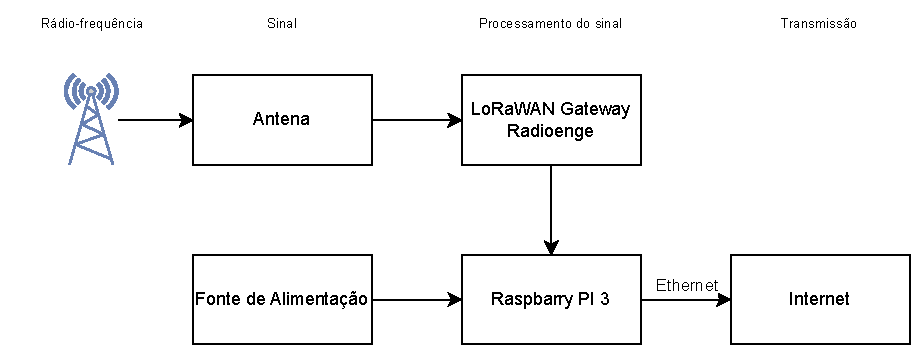
\includegraphics[width=1\linewidth]{assets/diagramaDeBlocoGateway.pdf}
    \caption{Diagrama de blocos do \textit{gateway LoRaWAN}.}
    \label{fig:diagrama_getway}
\end{figure}

\subsection{Servidor de Rede ChirpStack}
\label{sec:chirpstack}

Sobre o \textit{Raspberry Pi 3} foi instalado o \textit{ChirpStack}, servidor de rede \textit{LoRaWAN} de código aberto, responsável por autenticar os dispositivos, desduplicar os pacotes recebidos pelos \textit{gateways} e decodificar o \textit{payload}. Para tanto, configurou-se um decodificador (\textit{codec}) em \textit{JavaScript} que converte os 10 bytes recebidos no objeto estruturado descrito na Tabela~\ref{tab:payload}. Essa função, apresentada na Figura~\ref{fig:decoder}, valida o comprimento do quadro, expande a máscara de bits em indicadores por anomalia e remonta os inteiros de 16 bits a partir dos pares de bytes, disponibilizando o resultado no objeto \texttt{data.object}. Após a decodificação, o \textit{ChirpStack} publica cada evento de \textit{uplink} em um \textit{broker} \acs{MQTT} (\textit{Message Queuing Telemetry Transport}), tornando os dados disponíveis para consumo pela camada de aplicação. A adoção de um servidor de rede local, em vez de uma rede pública, garantiu controle total sobre o roteamento dos dados e maior previsibilidade na comunicação, requisitos importantes em uma aplicação clínica.

\begin{figure}[ht]
\centering
\begin{Verbatim}[fontsize=\small, frame=single]
function decodeUplink(input) {
  var b = input.bytes;
  if (!b || b.length < 10) return { errors: ["payload curto"] };
  var flags = b[0];
  return { data: {
    flags: flags,
    taqui:    (flags & 0x01) !== 0,
    bradi:    (flags & 0x02) !== 0,
    arritmia: (flags & 0x04) !== 0,
    bloqueio: (flags & 0x08) !== 0,
    parada:   (flags & 0x10) !== 0,
    bpm:       (b[1] << 8) | b[2],
    rrMed:     (b[3] << 8) | b[4],
    rrDp:      (b[5] << 8) | b[6],
    numPicos:   b[7],
    segmentId: (b[8] << 8) | b[9]
  }};
}
\end{Verbatim}
\caption{Função decodificadora (\textit{codec}) cadastrada no \textit{ChirpStack}, que converte o \textit{payload} de 10 bytes no objeto consumido pelo serviço de ingestão.}
\label{fig:decoder}
\end{figure}


\section{Ingestão e Persistência dos Dados}
\label{sec:ingestao}

A integração entre a infraestrutura \textit{LoRaWAN} e a aplicação foi realizada por um serviço de ingestão desenvolvido em \textit{Python}. Optou-se por uma arquitetura sem servidor de aplicação dedicado (\textit{serverless}): o único processo de retaguarda em execução contínua foi o ingestor, enquanto a persistência e a leitura dos dados ficaram a cargo de uma plataforma gerenciada em nuvem.

\subsection{Ingestor MQTT}
\label{sec:ingestor}

O ingestor inscreveu no \textit{broker} \acs{MQTT} do \textit{ChirpStack} e, a cada mensagem de \textit{uplink}, executa: a identificação do dispositivo de origem pelo seu \textit{DevEUI}; a verificação do paciente a ele vinculado; a determinação do tipo de evento de maior prioridade clínica a partir da máscara de \textit{flags}; e a gravação do evento cardíaco no banco de dados. Quando o evento é classificado como crítico, o ingestor registra também os eventos de alerta destinados aos profissionais de saúde ativos da respectiva instituição. Para conter o custo de operação da plataforma em nuvem, o serviço foi parametrizado de modo a permitir, opcionalmente, o descarte dos segmentos normais e a restrição das notificações apenas aos eventos críticos.

\subsection{Banco de Dados e Modelo de Dados}
\label{sec:bancoDados}

A persistência foi realizada no \textit{Cloud Firestore}, banco de dados de documentos (\acs{NoSQL}) da plataforma \textit{Firebase}, escolhido por oferecer sincronização em tempo real com os clientes, escalabilidade gerenciada e integração nativa com o serviço de autenticação. Por se tratar de um banco orientado a documentos, o modelo não é relacional: os dados foram organizados em coleções de documentos que se referenciam por meio de identificadores, adotando-se um modelo multi-instituição (\textit{multi-tenant}) em que cada documento referencia a entidade (instituição) à qual pertence. A Tabela~\ref{tab:colecoes} descreve as coleções e seus principais campos, e a Figura~\ref{fig:modeloFirestore} ilustra as referências entre elas.

\begin{table}[h]
    \centering
    \caption{Modelo de dados do \textit{Firestore}: coleções, principais campos e referências.}
    \small
    \begin{tabular}{l|>{\arraybackslash}m{6.7cm}|>{\arraybackslash}m{3.1cm}}
        \textbf{Coleção} & \textbf{Principais campos} & \textbf{Referências} \\ \hline
        \textit{entidades} & id, nome, ativo, criadoEm & --- \\ \hline
        \textit{usuarios} & id, nome, email, perfil, entidadeId, status, criadoEm & entidadeId $\rightarrow$ entidades \\ \hline
        \textit{pacientes} & id, nome, cpf, dataNascimento, ativo, entidadeId, criadoEm & entidadeId $\rightarrow$ entidades \\ \hline
        \textit{dispositivos} & id, devEui, entidadeId, pacienteId, cadastradoPor, criadoEm & entidadeId $\rightarrow$ entidades; pacienteId $\rightarrow$ pacientes \\ \hline
        \textit{eventosCardiacos} & id, dispositivoId, pacienteId, entidadeId, bpm, flags, tipoEvento, rrMed, rrDp, numPicos, segmentId, sinalCritico, origem, criadoEm & pacienteId $\rightarrow$ pacientes; dispositivoId $\rightarrow$ dispositivos \\ \hline
        \textit{notificacoes} & id, usuarioId, entidadeId, titulo, mensagem, lida, eventoId, criadoEm & usuarioId $\rightarrow$ usuarios; eventoId $\rightarrow$ eventosCardiacos \\ \hline
    \end{tabular}
    \label{tab:colecoes}
\end{table}

\begin{figure}[ht]
    \centering
    \begin{tikzpicture}[
        >={Stealth[round]},
        coll/.style={draw, rounded corners, fill=gray!12, align=center, minimum height=0.9cm, minimum width=2.9cm, font=\small},
        card/.style={font=\scriptsize}
    ]
        \node[coll] (ent)   at (0,0)      {entidades};
        \node[coll] (usr)   at (-4.3,-2)  {usuarios};
        \node[coll] (pac)   at (0,-2)     {pacientes};
        \node[coll] (disp)  at (4.3,-2)   {dispositivos};
        \node[coll] (evt)   at (2.0,-4)   {eventosCardiacos};
        \node[coll] (notif) at (-4.3,-4)  {notificacoes};

        \draw[->] (ent)  -- (usr)   node[card, midway, sloped, above]{1..N};
        \draw[->] (ent)  -- (pac)   node[card, midway, right]{1..N};
        \draw[->] (ent)  -- (disp)  node[card, midway, sloped, above]{1..N};
        \draw[->] (disp) -- (pac)   node[card, midway, above]{0..1};
        \draw[->] (pac)  -- (evt)   node[card, midway, sloped, below]{1..N};
        \draw[->] (evt)  -- (notif) node[card, midway, above]{1..N};
        \draw[->] (usr)  -- (notif) node[card, midway, left]{1..N};
    \end{tikzpicture}
    \caption{Modelo de dados do \textit{Firestore}: as setas indicam as referências entre coleções e a respectiva cardinalidade.}
    \label{fig:modeloFirestore}
\end{figure}

\subsection{Autenticação e Controle de Acesso}
\label{sec:seguranca}

A autenticação dos usuários foi delegada ao \textit{Firebase Authentication}. O controle de acesso baseou-se em regras de segurança (\textit{security rules}) declaradas no próprio \textit{Firestore}, que constituíram a única camada de autorização do cliente, dispensando um servidor intermediário. As regras determinam o perfil de cada usuário (administrador geral, administrador de instituição ou profissional de saúde) e seu estado de vínculo (pendente, ativo ou inativo) a partir do próprio documento do usuário, restringindo cada operação de leitura e escrita ao escopo da instituição correspondente. Dessa forma, garantiu-se o isolamento dos dados entre instituições distintas e a confidencialidade das informações clínicas. Os eventos gravados pelo ingestor, por utilizarem credenciais administrativas, foram inseridos diretamente, sem submissão às regras do cliente.


\section{Aplicativo Móvel}
\label{sec:app}

A interface de acompanhamento foi desenvolvida como um aplicativo móvel multiplataforma, executável em \textit{Android} e \textit{iOS}, voltado aos profissionais de saúde. A escolha por uma aplicação móvel, em detrimento de uma interface exclusivamente \textit{web}, deveu-se à mobilidade exigida no ambiente da clínica e à possibilidade de envio de notificações \textit{push} diretamente ao dispositivo do profissional.

\subsection{Tecnologias e Arquitetura}
\label{sec:appArq}

O aplicativo foi construído com o \textit{framework} \textit{React Native}, por meio da plataforma \textit{Expo} e do sistema de rotas \textit{Expo Router}. A comunicação com o banco de dados foi estabelecida diretamente entre o aplicativo e o \textit{Firestore}, por meio do \acs{SDK} do \textit{Firebase}, sem a intermediação de uma \acs{API} \acs{REST} própria. A atualização da interface em tempo real foi obtida com o mecanismo de \textit{listeners} do \textit{Firestore} (\textit{onSnapshot}), que propaga automaticamente para os clientes qualquer alteração nos dados; assim, um novo evento cardíaco gravado pelo ingestor aparece instantaneamente no painel dos profissionais conectados.

\subsection{Funcionalidades}
\label{sec:appFunc}

O aplicativo contemplou os fluxos de autenticação (cadastro, \textit{login}, recuperação de senha e tela de espera por vínculo institucional) e um conjunto de funcionalidades organizadas por perfil de usuário:

\begin{itemize}
    \item \textbf{Painel (\textit{dashboard})}: visualização, em tempo real, dos eventos cardíacos detectados, com destaque para os de natureza crítica.
    \item \textbf{Gestão de pacientes}: cadastro, edição, consulta e remoção de pacientes vinculados à instituição.
    \item \textbf{Gestão de dispositivos}: cadastro de dispositivos e vínculo/desvínculo com os pacientes.
    \item \textbf{Administração}: gestão de instituições e de usuários, incluindo a ativação de profissionais pendentes, restrita aos perfis administrativos.
    \item \textbf{Regras de alarme}: configuração, por tipo de anomalia, da quantidade mínima de ocorrências exigida em uma janela recente de segmentos para que eventos já registrados sejam promovidos a alarme.
    \item \textbf{Notificações}: recebimento de alertas \textit{push} a cada alarme confirmado, viabilizado pelo serviço de notificações do \textit{Expo}.
\end{itemize}

Como mecanismo de redução de alarmes falsos, o aplicativo incorporou uma regra de confirmação por persistência baseada em janela deslizante. Todos os eventos detectados pelo dispositivo são gravados no banco de dados e exibidos no histórico; a regra atua apenas sobre sua promoção a alarme. Para cada classe de evento, o profissional pode configurar uma condição do tipo $X$ em $N$: por exemplo, exigir que a arritmia sinusal apareça em 10 dos últimos 10 segmentos de um mesmo paciente antes que um novo evento dessa classe seja sinalizado como alarme confirmado. A contagem incide sobre a máscara de anormalidades do segmento, e não sobre a classe atribuída pela regra de precedência (Seção~\ref{sec:resPipeline}): uma anomalia detectada em conjunto com outra mais grave perde o rótulo do evento, mas continua a alimentar o seu próprio contador. Confirmado um alarme, os segmentos por ele consumidos deixam de contar para o seguinte, o que institui um período refratário --- sob anomalia contínua, a repetição fica limitada a um alarme a cada $X$ segmentos, ou cerca de 5 minutos na configuração padrão da arritmia sinusal. Os limiares padrão foram ajustados conforme a gravidade clínica: a parada sinoatrial confirma-se com uma única ocorrência; o bloqueio sinoatrial, a taquicardia e a bradicardia exigem persistência em janelas curtas; e a arritmia sinusal, de menor especificidade, requer a janela inteira. Dessa forma, preservou-se o registro integral dos eventos, distinguindo a detecção de uma anomalia de sua promoção a alerta crítico.

A Tabela~\ref{tab:casosUso} sintetiza as funcionalidades do sistema sob a perspectiva dos três perfis de usuário, conforme as permissões definidas nas regras de segurança (Seção~\ref{sec:seguranca}).

\begin{table}[h]
    \centering
    \caption{Funcionalidades da aplicação por perfil de usuário.}
    \small
    \begin{tabular}{>{\arraybackslash}m{6.6cm}|c|c|c}
        \textbf{Funcionalidade} & \textbf{Profissional} & \textbf{Administrador} & \textbf{Super Admin.} \\ \hline
        Acompanhar o painel de eventos em tempo real & Sim & Sim & Sim \\ \hline
        Receber alertas de eventos críticos & Sim & Sim & Sim \\ \hline
        Cadastrar e consultar pacientes & Sim & Sim & Sim \\ \hline
        Editar e remover pacientes & --- & Sim & Sim \\ \hline
        Vincular dispositivo a paciente & Sim & Sim & Sim \\ \hline
        Cadastrar e remover dispositivos & --- & Sim & Sim \\ \hline
        Registrar evento manual & Sim & Sim & Sim \\ \hline
        Gerir usuários da instituição & --- & Sim & Sim \\ \hline
        Gerir instituições & --- & Própria & Todas \\ \hline
        Configurar regras de alarme & Sim & Sim & Sim \\ \hline
    \end{tabular}
    \label{tab:casosUso}
\end{table}


\section{Validação do Sistema}
\label{sec:validacao}

A validação do sistema foi conduzida de forma incremental, acompanhando o desenvolvimento de cada componente. A integridade do sinal adquirido foi verificada por meio de uma ferramenta de visualização em tempo real, que recebeu as três derivações pela interface serial do dispositivo e as exibiu graficamente, permitindo avaliar a presença das ondas características do \acs{ECG} e a atuação dos filtros digitais. Um modo de diagnóstico do \textit{firmware} possibilitou alternar entre a saída do sinal bruto e a do sinal filtrado, bem como mensurar a taxa de amostragem efetiva do conversor. A consistência entre a detecção realizada na borda e os eventos persistidos em nuvem foi conferida por meio de comandos de despejo dos registros locais via interface serial, confrontando-os com os dados gravados no \textit{Firestore}.

\subsection{Validação com Gerador de Sinais Padrão}
\label{sec:validacaoGerador}

Para avaliar objetivamente a cadeia de processamento e transmissão, isolando-a da variabilidade inerente à aquisição por eletrodos no corpo, empregou-se um gerador de sinais arbitrários (\textit{National Instruments} myDAQ, operado pelo \textit{software} NI-ELVISmx) como fonte de sinais de \acs{ECG} de classe conhecida. Os sinais foram reproduzidos na saída analógica do gerador e injetados nos condutores de entrada do dispositivo, no lugar dos eletrodos. Como a saída do gerador opera na ordem de volts, acima da amplitude usual do \acs{ECG}, interpôs-se um divisor de tensão resistivo entre a saída analógica e o conector de entrada do dispositivo, conforme o arranjo da Figura~\ref{fig:bancadaGerador}. A geração em volts, seguida de atenuação junto à entrada, foi preferida à geração direta em milivolts porque preserva a forma de onda bem acima do ruído próprio do conversor do gerador.

Todos os arquivos de estímulo foram construídos com a mesma excursão --- pico de 0{,}97~V e vale de $-0{,}24$~V, ou seja, 1{,}21~V pico a pico ---, de modo que uma única calibração do atenuador vale para todas as classes ensaiadas. Com ganho unitário na saída do gerador, a amplitude medida na entrada do \acs{AFE} foi de aproximadamente 0{,}6~mV pico a pico, valor reproduzido em todas as baterias e correspondente a uma atenuação efetiva da ordem de 2.000:1, aferida pela razão entre a excursão aplicada e a amplitude adquirida. Esse nível situa-se abaixo da faixa de 1 a 2~mV típica da derivação II, de modo que os ensaios transcorreram em regime de relação sinal-ruído mais desfavorável que o esperado em uso clínico, o que confere caráter conservador aos resultados obtidos. A ausência de saturação foi verificada por meio da ferramenta de visualização. Cabe registrar que a conversão de contagens do conversor para milivolts foi derivada dos parâmetros de projeto do \acs{AFE}, sem aferição contra instrumento de referência; eventual erro nessa escala afeta apenas o eixo de amplitude das figuras, e não a classificação, uma vez que o detector opera sobre intervalos R-R e sobre limiares proporcionais à amplitude do próprio segmento.


\begin{figure}[H]
    \centering
    \begin{tikzpicture}[
        >={Stealth[round]},
        box/.style={draw, rounded corners, align=center, minimum height=1.5cm, font=\small},
        lbl/.style={font=\footnotesize, align=center},
        node distance=2.4cm
    ]
        \node[box, text width=3.9cm] (pc)  {Computador\\(NI-ELVISmx /\\ \texttt{\small bancada\_auto.py})};
        \node[box, right=of pc,  text width=2.8cm] (daq) {myDAQ\\gerador de sinais\\arbitrários};
        \node[box, right=of daq, text width=2.8cm] (div) {Divisor de tensão\\resistivo};
        \node[box, below=2.4cm of div, text width=3.4cm] (prot) {Protótipo\\ADS1293 + XIAO ESP32-S3\\(detecção na borda)};

        \draw[->] (pc)  -- (daq) node[midway, above, lbl]{USB\\(NI-DAQmx)};
        \draw[->] (daq) -- (div) node[midway, above, lbl]{AO0 / AGND\\$\approx$1,21~V\\pico a pico};
        \draw[->] (div) -- (prot) node[midway, right, lbl]{~3 fios\\~(RA, LA, LL)};

        % retorno pela serial: armamento do segmento e captura dos resultados
        \coordinate (r1) at (pc.south |- prot.west);
        \draw[->] (prot.west) -- (r1)
              node[midway, below, lbl]{Serial USB: armamento do segmento (comando \texttt{S}),\\captura dos resumos e dos segmentos brutos}
              -- (pc.south);
    \end{tikzpicture}
    \caption{Arranjo da bancada de validação com gerador de sinais. O computador reproduz o arquivo de estímulo na saída analógica do myDAQ, cuja tensão, na ordem de volts, é atenuada por um divisor resistivo antes de ser aplicada aos três condutores de entrada do protótipo, no lugar dos eletrodos. O mesmo computador arma e lê o dispositivo pela interface serial, o que permite alinhar o segmento analisado ao início da reprodução. O enlace de rádio permaneceu desativado durante as baterias, uma vez que a coleta automatizada exige o comando do processamento pela serial.}
    \label{fig:bancadaGerador}
\end{figure}

O teste foi conduzido como uma sucessão de \textit{baterias} de ensaios. Em cada bateria, para cada uma das seis classes --- normal, taquicardia, bradicardia, arritmia sinusal, bloqueio sinoatrial e parada sinoatrial ---, uma forma de onda representativa, de classe e frequência cardíaca conhecidas (gabarito), foi reproduzida no gerador, e o \textit{firmware} processou 30 segmentos de 30~s, totalizando 180 ensaios por bateria.

A reprodução obedeceu a dois protocolos sucessivos. Nas primeiras baterias, o arquivo de estímulo foi reproduzido de modo contínuo, em laço, e o \textit{firmware} processou 30 segmentos consecutivos. Nesse regime, o instante em que o gerador retorna ao início do arquivo --- a \textit{emenda} do laço --- recai dentro de um dos segmentos e cria um intervalo R-R que não corresponde a nenhum par de batimentos do estímulo. Ainda que o comprimento de cada arquivo tenha sido ajustado para conter um número inteiro de ciclos, o artefato persistiu sempre que a cauda diastólica não coincidiu com o intervalo mediano, e mostrou-se dominante entre as falhas das primeiras baterias, conforme analisado na Seção~\ref{sec:resValidacaoGerador}. A partir da sétima bateria adotou-se, por essa razão, o protocolo de \textbf{disparo único}: cada repetição é uma reprodução independente do arquivo, escrita na saída analógica em modo finito, precedida de 5~s de pré-reprodução --- necessários à estabilização do filtro passa-alta de 0,5~Hz --- e seguida de 1~s de folga, com o segmento do \textit{firmware} armado por comando enviado pela interface serial no instante do disparo. Como não há laço, não há emenda, e o segmento analisado fica alinhado ao início da reprodução. As baterias que medem o desempenho do sistema (Seção~\ref{sec:resValidacaoFinal}) empregam exclusivamente esse segundo protocolo; as conduzidas em reprodução contínua são relatadas por documentarem o percurso de depuração, e não como medida de desempenho.

Para cada segmento, a classe detectada pelo \textit{firmware} e o \textit{payload} de 10 bytes por ele montado foram confrontados com o sinal conhecido, verificando se a anomalia foi corretamente identificada e codificada no \textit{payload}. Ambos foram obtidos pela interface serial do dispositivo, uma vez que a coleta automatizada requer que o processamento do segmento seja iniciado por comando, o que impôs manter o enlace de rádio desativado durante os ensaios. A transmissão foi, por essa razão, validada de forma independente das baterias, confrontando-se o \textit{payload} publicado pelo servidor de rede com o evento persistido no banco e exibido no aplicativo (Seção~\ref{sec:resPipeline}).

O desempenho de cada bateria foi expresso por uma matriz de confusão entre a classe esperada e a detectada, da qual se derivaram a acurácia global e, por classe, no esquema um-contra-todos, a sensibilidade, a especificidade e os valores preditivos positivo e negativo. As classes sem estímulo esperado em uma dada bateria foram omitidas da respectiva matriz, e não reportadas com métricas degeneradas. A estimativa da frequência cardíaca foi avaliada à parte, pelo erro absoluto médio, em batimentos por minuto, entre o valor transmitido no \textit{payload} e o do sinal conhecido. Adotaram-se as mesmas métricas do trabalho que fundamentou o algoritmo de detecção (Seção~\ref{sec:deteccaoBorda}), de modo a tornar os resultados diretamente comparáveis.

O emprego de baterias sucessivas decorreu da necessidade de distinguir limitações dos sinais de classes connhecidas das limitações do próprio detector. As primeiras baterias empregaram formas de onda extraídas diretamente de registros de \acs{ECG} reais (classes de ritmo) e de sinais sintéticos contendo as pausas características (classes de bloqueio e parada sinoatrial, escassas nas bases públicas). O refinamento progressivo dos sinais e da cadeia de aquisição --- descrito em detalhe, com seus resultados, na Seção~\ref{sec:resValidacaoGerador} --- percorreu duas etapas. Na primeira, construiu-se um conjunto próprio, em que a morfologia dos batimentos veio de um molde extraído de um \acs{ECG} real cedido pelo orientador --- a média alinhada de seus batimentos --- e o ritmo foi imposto por síntese, distante dos limiares de decisão: intervalo R-R de 800~ms (75~bpm) no traçado normal, 500~ms (120~bpm) na taquicardia e 1.200~ms (50~bpm) na bradicardia, com variabilidade batimento a batimento de desvio-padrão de 15, 10 e 20~ms, respectivamente --- bem abaixo do limiar de 120~ms do critério de arritmia sinusal, para não induzir classe falsa. Sobre esse ritmo somaram-se imperfeições de amplitude, todas referidas à amplitude da onda R: deriva senoidal de linha de base de 5\,\%, modulação respiratória de $\pm$8\,\% e ruído branco de desvio-padrão de 2\,\%, sendo a modulação respiratória destinada a exercitar o limiar global de amplitude do detector. Na segunda etapa, a revisão do critério de pausa (Seção~\ref{sec:resRevisaoCriterio}) tornou os arquivos originais do orientador diretamente utilizáveis nas seis classes, e as baterias que medem o desempenho do sistema passaram a empregá-los sem qualquer sinal sintetizado ou derivado nesta dissertação.

A reprodução em laço impôs uma restrição adicional à construção dos arquivos: a junção entre o fim e o início (\textit{emenda}) não podia introduzir um intervalo R-R espúrio. Por isso cada arquivo foi truncado no último ciclo cardíaco completo, e as imperfeições periódicas foram geradas com número inteiro de ciclos ao longo da duração do arquivo --- 300~s, e não os 30~s do segmento analisado: oito ciclos de deriva de linha de base e vinte de modulação respiratória. Ressalve-se que a condição de ciclos inteiros refere-se ao comprimento do arquivo, e não ao segmento: um R-R de 800~ms, por exemplo, não perfaz número inteiro de ciclos em 30~s, mas perfaz 375 ciclos exatos em 300~s. A precaução tornou-se dispensável com o protocolo de disparo único.

A taxa de reprodução do gerador foi ajustada, em cada ensaio, à taxa em que o respectivo arquivo havia sido criado, de modo a preservar a base de tempo da forma de onda e, com ela, a duração dos intervalos R-R do sinal conhecido: reproduzir um arquivo em taxa diferente daquela em que foi gerado comprime ou dilata o traçado e desloca a frequência cardíaca de referência. Os arquivos cedidos pelo orientador foram criados a 500 amostras por segundo; nas primeiras baterias foram reamostrados para 640 amostras por segundo antes da reprodução e, a partir da sétima bateria, passaram a ser reproduzidos na taxa original, sem reamostragem. Os arquivos sintetizados neste trabalho foram gerados e reproduzidos a 640 amostras por segundo. Não há exigência de que a taxa do gerador coincida com a do conversor do dispositivo: a geração e a aquisição são processos independentes, e a hipótese de que o descasamento entre ambas produzisse modulação indesejada de amplitude foi expressamente testada e descartada (Seção~\ref{sec:resNotch}). Antes de cada bateria, a integridade da aquisição foi verificada pelo modo de diagnóstico do \textit{firmware}, confirmando a ausência de perda de amostras ao longo do segmento — controle que se mostrou determinante, conforme discutido na Seção~\ref{sec:resValidacaoGerador}.

